
\documentclass[12pt,letterpaper,oneside]{report}

% -------------------------- CONFIGURACIÓN GENERAL ----------------------------

% Idioma y codificación
\usepackage[spanish]{babel}
\usepackage[utf8]{inputenc}
\usepackage[T1]{fontenc}

% Bibliografía APA 7ma edición
\usepackage[style=apa,backend=biber,sortcites=true,sorting=nyt,hyperref=true]{biblatex}
\DeclareLanguageMapping{spanish}{spanish-apa}
\addbibresource{referencias.bib}

% Sangría francesa y espacio entre referencias para APA
\setlength{\bibhang}{1.27cm} % sangría francesa recomendada por APA
\setlength{\bibitemsep}{1.2\baselineskip} % espacio entre referencias (opcional)

% Márgenes y papel carta (2.54 cm estándar)
\usepackage{geometry}
\geometry{
  paper=letterpaper,
  left=2.54cm,
  right=2.54cm,
  top=2.54cm,
  bottom=2.54cm
}

% Paquetes de matemáticas y símbolos
\usepackage{amsmath,amssymb}

% Gráficos y tablas
\usepackage{graphicx}
\graphicspath{{images/}}
\usepackage{booktabs}
\usepackage{array}
\usepackage{longtable}
\usepackage{tikz}
\usetikzlibrary{arrows.meta, positioning, shapes.geometric}

% Hipervínculos y formato de referencias
\usepackage[colorlinks=true, linkcolor=black, urlcolor=blue, citecolor=black, pdfborder={0 0 0}]{hyperref}

% Formato de captions para tablas y figuras
\usepackage{caption}
\captionsetup[table]{labelfont=bf}
\captionsetup[figure]{labelfont=bf}
\captionsetup[figure]{labelformat=default,labelsep=period,name=Figura}
\captionsetup[table]{labelformat=default,labelsep=period,name=Tabla}

% Listas y apéndices
\usepackage{enumitem}
\usepackage{appendix}

% Encabezados y pie de página
\usepackage{fancyhdr}

% Citas con biblatex (requerido para APA 7ma)
\usepackage{csquotes}

% Cambiar nombre de Tabla de Contenido y listas (ajustar según idioma)
\addto\captionsspanish{
  \renewcommand{\contentsname}{Tabla de Contenido}
  \renewcommand{\listfigurename}{Lista de Figuras}
  \renewcommand{\listtablename}{Lista de Tablas}
  \renewcommand{\figurename}{Figura}
  \renewcommand{\tablename}{Tabla}
}

% Archivo de estilo personalizado con títulos (CRÍTICO: NO quitar)
\usepackage{estiloUNAD}

% Configuración de sangría y espacio entre párrafos
\setlength{\parindent}{1.5em}
\setlength{\parskip}{0.5em}

% Si se desea personalizar la lista de contenido, descomentar:
% \usepackage{tocloft}

% -------------------------- INICIO DEL DOCUMENTO ----------------------------

\begin{document}

% Numeración de tablas y figuras continua a lo largo del documento (CRÍTICO para formatos de tesis)
\renewcommand{\thefigure}{\arabic{figure}}
\renewcommand{\thetable}{\arabic{table}}
\counterwithout{figure}{chapter}
\counterwithout{table}{chapter}

% Portada y preliminares (estos archivos deben estar presentes)
% ========================================================================
%                     PORTADA Y CONTRAPORTADA
% Los datos se toman de main.tex (sección "DATOS DEL TRABAJO").
% ========================================================================

% ------------------------------- Portada --------------------------------
\begin{titlepage}
\thispagestyle{empty}
\begin{center}
\singlespacing
% Si su programa exige el logo, guárdelo en figuras/ y descomente:
% \includegraphics[width=4cm]{logo-unab}\par\vspace{1cm}

\vspace*{2cm}
{\bfseries \tituloTrabajo\par}

\vfill
\autores\par

\vfill
\universidad\\
\facultad\\
\programa\\
\ciudad\\
\anio
\end{center}
\end{titlepage}

% ---------------------------- Contraportada -----------------------------
\begin{titlepage}
\thispagestyle{empty}
\begin{center}
\singlespacing
\vspace*{2cm}
{\bfseries \tituloTrabajo\par}

\vfill
\autores\par

\vfill
Trabajo de grado presentado como requisito para optar al título de\\
\tituloProfesional

\vfill
Director:\\
\director\\
\directorFormacion\\
\directorAfiliacion

\vspace{0.8cm}
Codirector:\\
\codirector\\
\codirectorFormacion\\
\codirectorAfiliacion

\vfill
\universidad\\
\facultad\\
\programa\\
\ciudad\\
\anio
\end{center}
\end{titlepage}

\begin{titlepage}
    \thispagestyle{empty} % Sin número de página

    \begin{center}
        \vspace*{1.7cm}
        \textbf{Nota de Aceptación}

        \vspace{0.8cm}
        \raggedright
        Esta página es opcional
        \par
        \vspace{2.0cm}
        \centering

        \rule{7cm}{0.4pt} \\ % Línea horizontal
        Nombre Director de Trabajo de Grado

        \vspace{3.0cm}

        \noindent
        \rule{5cm}{0.4pt}\hfill\rule{5cm}{0.4pt} \\[0.2cm]
        \hspace{0.5cm}Jurado\hfill\hspace{-1cm}Jurado

        \vspace{5.0cm}

        2025
    \end{center}
\end{titlepage}
\begin{titlepage}
    \thispagestyle{empty}
    \begin{center}
        \vspace*{2cm}
        \textbf{Dedicatoria}
        
        \vspace{0.8cm}
        Aún no.
        
        \vspace{15cm}
    \end{center}
\end{titlepage}
\clearpage
    \thispagestyle{plain}
    \phantomsection
    \begin{center}
        \vspace*{2cm}
        \textbf{Agradecimientos}
        
        \vspace{0.8cm}
        \textit{[Sección opcional, pendiente de decisión de los autores.]}
        
        \vspace{15cm}
    \end{center}
\clearpage

\chapter*{Resumen}
\phantomsection
    Las lesiones cutáneas malignas plantean un reto diagnóstico, especialmente en contextos donde escasean los datos clínicos etiquetados y los conjuntos públicos proceden de poblaciones distintas a la de Santander. Este trabajo desarrolla un algoritmo de clasificación de lesiones cutáneas mediante aprendizaje autosupervisado y estudia, como líneas complementarias, la segmentación y la transformación y estimación del tono de piel. En la comparación congelada sobre HAM10000, los intervalos bootstrap pareados del 95\,\% de B71 frente a ocho líneas base excluyeron cero; estos contrastes no tuvieron una corrección global por multiplicidad y se interpretan dentro de esa familia. La adaptación con imágenes sin etiquetas de PAD-UFES-20 mostró una mejora piloto frente al control de cómputo, aunque el modelo adaptado permaneció por debajo del codificador público. La variante S4-A2 obtuvo Dice de 0,7221 en ISIC2018 y 0,7949 en HAM10000, sin demostrar una mejora general del clasificador al integrar máscaras. En la evaluación propia de PAD-UFES-20, el estimador ITA quedó por debajo de la línea base por mayoría. Los resultados son experimentales y no constituyen validación clínica ni evidencia de representatividad regional. La implementación del prototipo previsto en el objetivo 4 sigue pendiente mientras se seleccionan el modelo y la configuración finales.
    \vspace{0.5cm}
    \textit{Palabras clave:} aprendizaje autosupervisado, SimSiam, DINOv2, clasificación de lesiones cutáneas, adaptación de dominio, segmentación de lesiones, estimación del tono de piel.

\chapter*{Abstract}
\phantomsection
    Malignant skin lesions pose a diagnostic challenge, particularly in settings with limited labeled clinical data and public datasets collected from populations that differ from Santander. This study develops a self-supervised skin lesion classification algorithm and examines segmentation and skin-tone transformation and estimation as complementary workstreams. In the frozen comparison on HAM10000, the paired bootstrap 95\% confidence intervals for B71 versus eight baselines excluded zero. These contrasts were not subject to a global multiplicity correction and are interpreted within that comparison family. Adaptation using unlabeled PAD-UFES-20 images showed a pilot improvement over the compute-matched control, although the adapted model remained below the public encoder. S4-A2 achieved Dice scores of 0.7221 on ISIC 2018 and 0.7949 on HAM10000, without demonstrating an overall classifier improvement from mask integration. In the project’s PAD-UFES-20 evaluation, the ITA estimator remained below the majority-class baseline. The findings are experimental and do not constitute clinical validation or evidence of regional representativeness. Implementation of the prototype planned under objective 4 remains pending while the final model and configuration are selected.
    \vspace{0.5cm}
    \textit{Keywords:} self-supervised learning, SimSiam, DINOv2, skin lesion classification, domain adaptation, lesion segmentation, skin tone estimation.


% Índices automáticos
\tableofcontents
\newpage
\listoffigures
\newpage
\listoftables
\newpage

% Marcador provisional. La lista se completará cuando se definan los anexos.
\chapter*{Lista de apéndices}
\addcontentsline{toc}{chapter}{Lista de apéndices}
\noindent\textit{[Pendiente: enumerar los apéndices que se incorporen a la versión final.]}

% Cuerpo del anteproyecto
\chapter{Introducción}
Las lesiones cutáneas son alteraciones visibles de la piel que pueden originarse por factores genéticos, ambientales o como manifestación de enfermedades sistémicas. Su clasificación entre benignas y malignas es clínicamente fundamental, ya que determina el curso del tratamiento y el pronóstico del paciente. A pesar de su alta prevalencia a nivel mundial, su diagnóstico oportuno sigue siendo un reto, especialmente en regiones con acceso limitado a servicios especializados. Este proyecto propone el desarrollo de un prototipo de apoyo diagnóstico basado en aprendizaje autosupervisado, orientado a fortalecer las capacidades de identificación de lesiones cutáneas y reducir la dependencia de datos etiquetados en contextos clínicos con recursos limitados como Santander.

\chapter{Planteamiento del Problema}
Las lesiones cutáneas comprenden alteraciones benignas y malignas que requieren clasificación clínica. Entre las malignas se encuentran el melanoma, el carcinoma basocelular y el carcinoma escamocelular. La carga mundial del melanoma y del cáncer cutáneo no melanoma ha sido analizada para el periodo 1990--2021 \parencite{zhou2025skinburdengbd}. En Colombia, la Cuenta de Alto Costo reportó 11.064 casos atendidos de melanoma cutáneo hasta el 31 de diciembre de 2024; el dato era preliminar y estaba sujeto a auditoría \parencite{cuentaaltocosto2025melanoma}.

La evidencia epidemiológica local disponible incluye un estudio del carcinoma basocelular en el área metropolitana de Bucaramanga \parencite{uribe2018bccbucaramanga}. Las cifras adicionales atribuidas al Instituto de Cáncer del HIC —3.060 casos entre 2016 y 2023 y la proporción de mortalidad atribuida al melanoma— requieren una fuente institucional primaria que documente periodo, población y definición de caso. Se incorporará esa evidencia cuando se localice.

\noindent\textit{[Pendiente: recuperar la referencia completa de Oliveros et al. (2025) y verificar la población, el periodo y el método antes de incluir las cifras de incidencia por altitud. No interpretar la altitud como causa de incidencia sin respaldo del estudio.]}

La inspección clínica y la dermatoscopía requieren conocimiento especializado. Los modelos de clasificación de imágenes han mostrado resultados en conjuntos de datos de investigación, pero su rendimiento depende de la tarea, la población y el protocolo de evaluación; esos resultados no equivalen a validación clínica del presente prototipo \parencite{esteva2017dermatologist,tschandl2018ham10000}. Las afirmaciones sobre exactitud según años de experiencia, variabilidad entre especialistas, tiempos de espera o costos locales se mantienen fuera de la versión factual hasta contar con fuentes primarias compatibles.

\noindent\textit{[Pendiente: añadir evidencia local si se afirma escasez de dermatólogos o retrasos de atención en Santander.]}

Una barrera metodológica es la disponibilidad limitada de anotaciones clínicas, ya que su producción requiere tiempo de especialistas. El aprendizaje autosupervisado puede aprovechar imágenes no etiquetadas para aprender representaciones, pero la clasificación posterior continúa requiriendo etiquetas para entrenar o evaluar el clasificador lineal. Otra dificultad es el cambio de dominio: las imágenes de entrenamiento pueden diferir de las de aplicación por población, dispositivo, iluminación o protocolo de captura. La necesidad de evaluar la generalización entre centros también se ha observado en estudios de IA médica, aunque no todos se refieren a dermatología \parencite{yang2024crosshospital}.

Por ello, la pregunta central del proyecto es:

\begin{quote}
¿Cómo diseñar un algoritmo de inteligencia artificial basado en aprendizaje autosupervisado para clasificar lesiones cutáneas a partir de imágenes dermatológicas y apoyar el análisis clínico en el contexto del departamento de Santander?
\end{quote}

\section{Árbol del problema}
\noindent\textbf{[Pendiente de actualización.]}

Reformular el árbol para que el problema central describa la dificultad de clasificar lesiones cutáneas con modelos computacionales cuando hay pocas etiquetas clínicas y existe cambio de dominio. Verificar con evidencia antes de atribuir al departamento retrasos asistenciales, sobrecarga clínica, costos o mortalidad.





\chapter{Justificación}

El proyecto aborda un problema de investigación en visión por computador médica: aprender representaciones para clasificar lesiones cutáneas cuando las etiquetas clínicas son limitadas. El aprendizaje autosupervisado permite usar imágenes no etiquetadas durante la fase de representación y evaluar después cómo esas representaciones sirven para la tarea de clasificación \parencite{krishnan2022selfsupervisedmedicine}.

La contribución metodológica consiste en documentar y evaluar un clasificador SSL, compararlo con controles explícitos y comunicar sus límites. Los resultados se interpretarán en relación con el protocolo y el conjunto de datos usados; no se presentarán como diagnóstico, eficacia clínica ni mejora asistencial. La evidencia local de carcinoma basocelular ofrece contexto regional, pero no demuestra que HAM10000 represente la epidemiología completa de Santander \parencite{uribe2018bccbucaramanga,tschandl2018ham10000}.

El proyecto también permite estudiar, sin asumir de antemano que aporten al clasificador, módulos complementarios de segmentación, manejo de artefactos y estimación de tono. El flujo modular exige validarlos de forma independiente y medir su aporte incremental antes de integrarlos. Esta separación permite conservar hallazgos negativos o no concluyentes y evita atribuir al SSL mejoras que podrían deberse a cambios en los datos, la partición o el preprocesamiento.

La viabilidad se apoya en conjuntos de datos públicos de investigación, código reproducible y recursos institucionales de cómputo. El trabajo se delimita al experimento computacional y a un prototipo de laboratorio; no incluye recolección propia de imágenes, pruebas con pacientes ni despliegue hospitalario. La representatividad de los conjuntos, la comparabilidad con líneas base supervisadas y la incertidumbre estadística se tratarán como limitaciones, no como beneficios ya demostrados.





\chapter{Objetivos}

\section*{Objetivo General}
Analizar el impacto de [tema o fenómeno] en [grupo, área o contexto específico], con el fin de comprender sus principales causas, efectos y posibles soluciones.

\section*{Objetivos Específicos}
\begin{itemize}
    \item Identificar los factores que contribuyen al desarrollo de [tema o fenómeno] en [lugar o grupo específico], mediante la recopilación y análisis de información teórica y empírica.
    \item Identificar los factores que contribuyen al desarrollo de [tema o fenómeno] en [lugar o grupo específico], mediante la recopilación y análisis de información teórica y empírica.
    \item Identificar los factores que contribuyen al desarrollo de [tema o fenómeno] en [lugar o grupo específico], mediante la recopilación y análisis de información teórica y empírica.
\end{itemize}
\chapter{Alcance y delimitación del proyecto}

El alcance principal es el diseño y la evaluación experimental de un clasificador de lesiones cutáneas basado en aprendizaje autosupervisado. El clasificador es el módulo central del proyecto. La segmentación, el manejo de pelo/artefactos y la estimación de tono son módulos complementarios que se evalúan por separado; su integración con el clasificador requiere contratos de entrada/salida, gates aprobados y ablaciones que midan su aporte incremental.

HAM10000 constituye el conjunto etiquetado principal para la evaluación de clasificación de siete categorías: \texttt{nv}, \texttt{mel}, \texttt{bkl}, \texttt{bcc}, \texttt{akiec}, \texttt{vasc} y \texttt{df} \parencite{tschandl2018ham10000}. No contiene una clase independiente para carcinoma escamocelular invasor ni cubre patologías tropicales como leishmaniasis. El conjunto de preentrenamiento no supervisado y sus exclusiones se reportarán a partir de manifiestos y hashes de cada corrida. BCN20000 no se contará como un conjunto independiente cuando sus imágenes ya formen parte de ISIC2019.

PAD-UFES-20 se reporta como evaluación externa de dominio, sin ajuste del modelo, porque contiene imágenes clínicas capturadas con teléfonos y no es directamente comparable con la dermatoscopía de HAM10000 \parencite{pacheco2020padufes}. El informe describirá el protocolo, el mapeo de etiquetas y sus limitaciones. La pertenencia exacta de las imágenes a conjuntos, particiones y exclusiones se documentará con identificadores y hashes verificables.

El proyecto utiliza conjuntos públicos y no contempla la recolección de imágenes en hospitales ni la evaluación prospectiva con pacientes o profesionales clínicos. El prototipo se considera una demostración de laboratorio, no un dispositivo médico validado, una herramienta diagnóstica autónoma ni un sistema desplegado en una institución de salud. La validez externa, la representatividad regional y los análisis de subgrupos se limitarán a la evidencia observada y a la calidad de las anotaciones disponibles.





\chapter{Estado del arte}
\section{Titulo nivel 2}
La globalización ha generado una transformación significativa en la forma en que las sociedades interactúan, comparten información y desarrollan sus economías. Esta interconexión ha traído consigo múltiples beneficios, como el acceso a nuevas tecnologías y mercados, pero también ha planteado desafíos importantes en términos de identidad cultural, sostenibilidad y equidad. Comprender estos efectos resulta clave para formular estrategias que permitan un desarrollo más equilibrado y justo.

\subsection{Ejemplo de ubicación de viñetas}
\begin{itemize}
    \item •	Comprender estos efectos resulta clave para formular estrategias que permitan un desarrollo más equilibrado y justo.
    \item •	Comprender estos efectos resulta clave para formular estrategias que permitan un desarrollo más equilibrado y justo.
    \item •	Comprender estos efectos resulta clave para formular estrategias que permitan un desarrollo más equilibrado y justo.
\end{itemize}
\subsection{Titulo nivel 3}
El uso de herramientas digitales en entornos educativos ha demostrado un potencial considerable para mejorar el aprendizaje, especialmente en contextos donde el acceso a recursos tradicionales es limitado. Sin embargo, la brecha digital persiste como una barrera que impide una participación equitativa. Es necesario que las políticas públicas y las instituciones académicas trabajen conjuntamente para garantizar una inclusión real, promoviendo tanto la infraestructura como la capacitación adecuada.
\subsubsection{Titulo nivel 4}
El uso de herramientas digitales en entornos educativos ha demostrado un potencial considerable para mejorar el aprendizaje, especialmente en contextos donde el acceso a recursos tradicionales es limitado. Sin embargo, la brecha digital persiste como una barrera que impide una participación equitativa. Es necesario que las políticas públicas y las instituciones académicas trabajen conjuntamente para garantizar una inclusión real, promoviendo tanto la infraestructura como la capacitación adecuada.

\paragraph{Titulo nivel 5}
Uno de los aspectos más relevantes al analizar cualquier fenómeno social es la necesidad de integrar diferentes perspectivas disciplinarias. La complejidad de los problemas actuales requiere enfoques interdisciplinarios que consideren factores económicos, culturales, ambientales y tecnológicos. Solo así es posible alcanzar una comprensión más profunda de la realidad y proponer soluciones sostenibles y efectivas.
La complejidad de los problemas actuales requiere enfoques interdisciplinarios que consideren factores económicos, culturales, ambientales y tecnológicos. Solo así es posible alcanzar una comprensión más profunda de la realidad y proponer soluciones sostenibles y efectivas.
Uno de los aspectos más relevantes al analizar cualquier fenómeno social es la necesidad de integrar diferentes perspectivas disciplinarias. La complejidad de los problemas actuales requiere enfoques interdisciplinarios que consideren factores económicos, culturales, ambientales y tecnológicos. Solo así es posible alcanzar una comprensión más profunda de la realidad y proponer soluciones sostenibles y efectivas.

\chapter{Figuras}

\section*{Ejemplo de Figura con su Nota}

\begin{figure}[htbp]
    \centering
    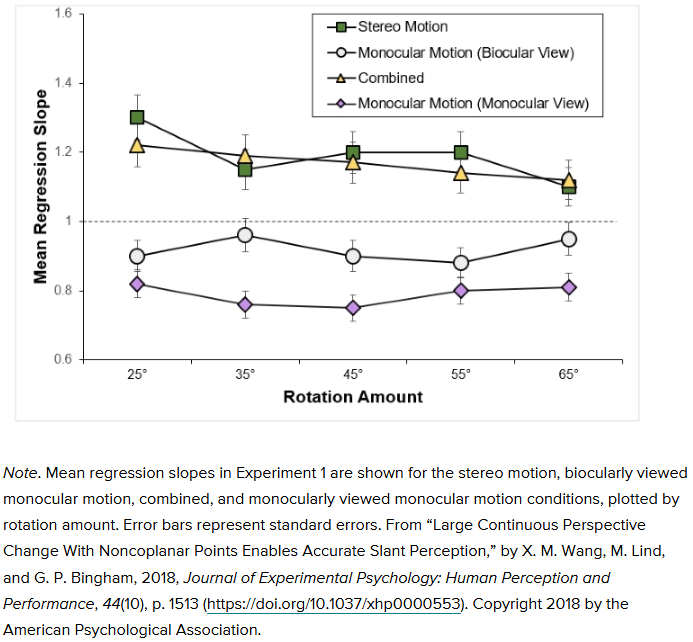
\includegraphics[width=0.75\textwidth]{image1.png}
    \caption{\textit{Pie de Figura}}
    \label{fig:ejemplo-nota}
\end{figure}

\textbf{Nota.} Se hace una descripción del contenido de la tabla en cuestión de lo que se esté exponiendo dentro de esta. Cuando la figura es de elaboración propia no es necesario agregar ningún tipo de declaración de derechos de autor. En APA se asume que todo lo que no tenga cita (o la declaración de derechos de autor) es de autoría del propio autor.

\chapter{Tablas}

\section*{}

\begin{table}[htbp]
     \caption{\textit{El Título Debe ser Breve y Descriptivo (en Cursiva)}}
    \centering
    \begin{tabular}{p{7cm} p{7cm}}
        \toprule
        \textbf{Columna uno} & \textbf{Columna dos} \\
        \midrule
        Table data & Table data \\
        Table data & Table data \\
        Table data & Table data \\
        Table data & Table data \\
        Table data & Table data \\
        \bottomrule
    \end{tabular}
\end{table}

% Nota APA debajo de la tabla, alineada a la izquierda
\noindent\textit{Nota.} Se hace una descripción del contenido de la tabla en cuestión de lo que se esté exponiendo dentro de esta, para referenciar la tabla se puede tomar el ejemplo de la figura que está ubicada en este documento.


% Source: Anteproyecto (3).pdf. Original wording retained except population/sample.
\chapter{Diseño metodológico}

El presente diseño metodológico establece la ruta estructurada que orientará el desarrollo del proyecto desde la identificación de los datos hasta el despliegue del prototipo funcional. El proyecto se enmarca en una investigación aplicada con enfoque cuantitativo y alcance experimental, cuyo propósito es el diseño e implementación de un modelo de inteligencia artificial basado en aprendizaje autosupervisado para el apoyo diagnóstico de lesiones cutáneas en contextos clínicos con escasez de datos etiquetados en el departamento de Santander.

El desempeño del modelo será cuantificado mediante métricas estándar de clasificación AUC-ROC, F1-score y exactitud que permiten comparaciones objetivas entre configuraciones (Hernández-Sampieri et al., 2018). Para garantizar la validez interna de las comparaciones, el modelo SSL será entrenado y sometido a ajuste de hiperparámetros manteniendo constantes el conjunto de datos, la arquitectura backbone y el protocolo de evaluación, contrastando los resultados obtenidos con modelos supervisados de referencia reportados en la literatura bajo las mismas condiciones experimentales.

\section{Diseño de la investigación}

El desarrollo del proyecto estará basado en el cumplimiento de los objetivos formulados siguiendo el modelo CRISP-ML(Q), estructurado originalmente en seis fases: comprensión del negocio y de los datos, ingeniería de datos, ingeniería del modelo, evaluación del modelo, despliegue y monitoreo continuo, Estas fases se agrupan en cuatro etapas iterativas representadas en la Figura~\ref{fig:original-10}: (i) Comprensión del problema clínico y de los datos dermatológicos, (ii) Ingeniería de datos y modelado del algoritmo SSL, (iii) Evaluación del modelo con aseguramiento de calidad y (iv) Implementación y despliegue del prototipo de apoyo al diagnóstico clínico. La sexta fase del modelo original, correspondiente al monitoreo y mantenimiento del modelo en producción, excede el nivel de madurez tecnológica TRL 4 proyectado para este trabajo de grado; por esta razón, se documenta como línea de continuidad para investigaciones posteriores.

\begin{figure}[htbp]
    \centering
    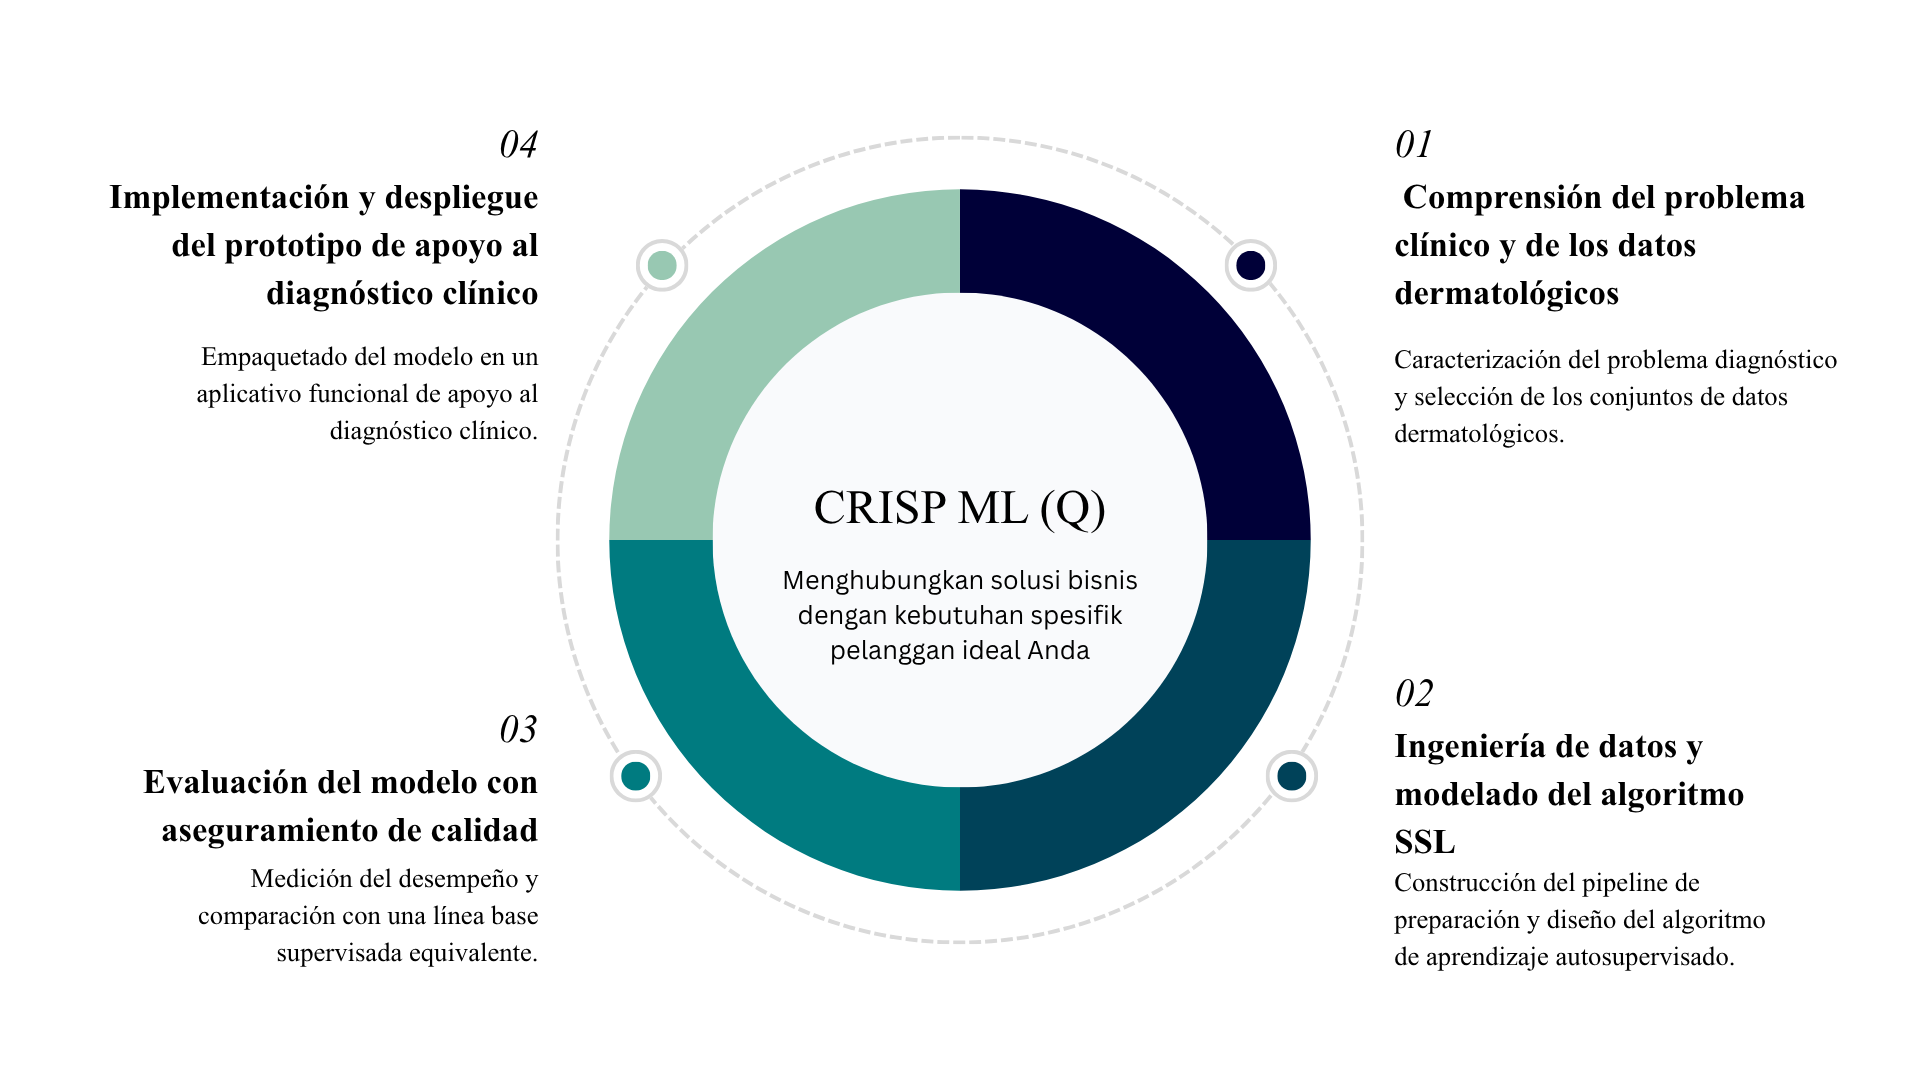
\includegraphics[width=0.9\textwidth]{figura10-diseno-crisp-mlq.png}
    \caption{Diseño metodológico basado en CRISP-ML(Q)}
    \label{fig:original-10}
\par\smallskip
\raggedright\footnotesize
\textit{Nota.} Creación propia.
\end{figure}

\section{Población y muestra}

La disponibilidad de conjuntos de datos de imágenes dermatológicas con fines investigativos es reducida en el contexto clínico del departamento de Santander. Ante esta restricción, el estudio adopta repositorios públicos consolidados en la literatura de clasificación dermatológica. La población de análisis corresponde a las imágenes dermatológicas disponibles en los conjuntos seleccionados; su uso no constituye una muestra representativa de pacientes del departamento ni una validación clínica regional.

HAM10000 es el conjunto fuente para el entrenamiento del clasificador y para la selección, calibración y evaluación interna, con sus siete categorías diagnósticas \parencite{tschandl2018ham10000}. Las particiones deben mantener cada lesión identificada por \texttt{lesion\_id} dentro de un único subconjunto para prevenir la fuga entre entrenamiento, validación y prueba. Los tamaños efectivos de la muestra y de las particiones se documentarán mediante los manifiestos de cada experimento, sin asumir que todas las imágenes disponibles se utilizan en cada fase.

PAD-UFES-20 se reserva para la evaluación externa del modelo \parencite{pacheco2020padufes}. Sus imágenes clínicas capturadas con teléfonos móviles difieren de las imágenes dermatoscópicas de HAM10000, de modo que esta evaluación estudia la transferencia entre modalidades y dominios. PAD-UFES-20 no se utiliza para el entrenamiento, la selección de modelos o hiperparámetros, la calibración ni el ajuste de umbrales. Se documentarán el mapeo de etiquetas, las clases compatibles y las limitaciones de la comparación.

La selección de imágenes estará guiada por criterios de calidad y pertinencia diagnóstica, aplicados de forma diferenciada según la fuente. La procedencia, las etiquetas disponibles, las licencias, los criterios de inclusión y exclusión y el preprocesamiento se registrarán junto con los identificadores y hashes de las particiones. La composición del conjunto de imágenes no etiquetadas para preentrenamiento se reportará conforme a los manifiestos y exclusiones de cada corrida, evitando incorporar imágenes reservadas para selección o prueba.

\section{Fases de la investigación}

\subsection{Fase 1 -- Comprensión del problema clínico y de los datos dermatológicos}

En esta fase se desarrolla la comprensión integral del problema diagnóstico de lesiones cutáneas en el contexto del departamento de Santander y se realiza la caracterización de los conjuntos de datos públicos de imágenes dermatológicas que sustentarán el desarrollo del modelo. Se evalúan aspectos relacionados con la incidencia y prevalencia epidemiológica de las lesiones cutáneas reportadas a nivel regional, las propiedades estadísticas de los datasets candidatos --distribución de clases, calidad de imagen, tamaño y condiciones de licencia-- y la matriz de riesgos por fase que orientará las etapas posteriores del proyecto, en concordancia con los componentes de aseguramiento de calidad (Q) propuestos por Studer et al. (2021). Entregable: Informe de comprensión empresarial y de datos con la caracterización formal de los conjuntos de datos seleccionados, los criterios de inclusión y exclusión, las métricas objetivo del modelo y la matriz de riesgos por fase.

Actividad 1.1: Revisar literatura científica y reportes epidemiológicos relacionados con lesiones cutáneas de mayor relevancia clínica en el departamento de Santander.

Actividad 1.2: Definir los objetivos de aprendizaje automático del proyecto y traducirlos a métricas medibles, en concordancia con el perfil epidemiológico regional y los estándares reportados en la literatura.

Actividad 1.3: Identificar y caracterizar conjuntos de datos públicos de imágenes dermatológicas, documentando tamaño, calidad de imagen, distribución de clases, fototipos representados y condiciones de licencia.

Actividad 1.4: Seleccionar las imágenes y clases diagnósticas pertinentes para el contexto del proyecto, aplicando criterios de inclusión y exclusión previamente definidos.

Actividad 1.5: Consolidar la matriz de riesgos por fase y los criterios de aseguramiento de calidad (Q) que orientarán el desarrollo de las fases posteriores.

\subsection{Fase 2 -- Ingeniería de datos y modelado del algoritmo SSL}

En esta fase se desarrolla el pipeline reproducible de preparación de los datos seleccionados en la fase anterior y se diseña el algoritmo de clasificación basado en aprendizaje autosupervisado. El proceso incluye la implementación de las transformaciones de preprocesamiento, la partición estratificada de los conjuntos de datos, la selección de la arquitectura backbone, el entrenamiento autosupervisado con imágenes no etiquetadas y el ajuste fino supervisado, manteniendo un registro completo de metadata de cada experimento para garantizar la reproducibilidad de los resultados. Entregable: Pipeline de datos versionado y algoritmo computacional basado en aprendizaje autosupervisado para la clasificación de lesiones cutáneas, con documentación de arquitectura, hiperparámetros y trazabilidad experimental.

Actividad 2.1: Implementar el pipeline de preprocesamiento de imágenes, incluyendo redimensionamiento, normalización, aumento de datos y partición estratificada en subconjuntos de entrenamiento, validación y prueba.

Actividad 2.2: Revisar modelos y estrategias de aprendizaje autosupervisado reportadas en la literatura para clasificación de imágenes médicas y dermatológicas.

Actividad 2.3: Seleccionar la arquitectura base (backbone) y definir la estrategia de entrenamiento autosupervisado del modelo propuesto.

Actividad 2.4: Entrenar el modelo mediante aprendizaje autosupervisado utilizando imágenes dermatológicas sin etiquetas y realizar el ajuste fino supervisado sobre el conjunto de datos etiquetados.

Actividad 2.5: Documentar la arquitectura final del modelo, los hiperparámetros utilizados, las decisiones de diseño adoptadas y la metadata completa de los experimentos realizados.

\subsection{Fase 3 -- Evaluación del modelo con aseguramiento de calidad}

En esta fase se evalúa el desempeño del algoritmo propuesto mediante métricas estándar de clasificación dermatológica reportadas en la literatura científica y se realiza una comparación experimental con modelos supervisados de referencia entrenados bajo las mismas condiciones experimentales. Adicionalmente, se incorporan los componentes de aseguramiento de calidad (Q) propios del marco CRISP-ML(Q), incluyendo el análisis de robustez del modelo, la auditoría de fairness por fototipo de piel y la generación de mapas de explicabilidad. Entregable: Informe comparativo con métricas de desempeño, matrices de confusión, análisis estadístico, auditoría de fairness y mapas de explicabilidad del modelo propuesto frente a los modelos supervisados de referencia.

Actividad 3.1: Identificar y seleccionar modelos supervisados de referencia reportados en la literatura científica para comparación experimental.

Actividad 3.2: Implementar los modelos de referencia utilizando el mismo conjunto de datos, backbone y protocolo experimental del modelo propuesto.

Actividad 3.3: Calcular métricas de evaluación como AUC-ROC, F1-score, exactitud, precisión y sensibilidad, desagregando los resultados por clase diagnóstica.

Actividad 3.4: Realizar análisis de robustez del modelo, auditoría de fairness por fototipo de piel y generación de mapas de explicabilidad como componentes de aseguramiento de calidad.

Actividad 3.5: Elaborar el análisis estadístico y la documentación comparativa de los resultados obtenidos durante la evaluación experimental.

\subsection{Fase 4 -- Implementación y despliegue del prototipo de apoyo al diagnóstico clínico}

En esta fase se desarrolla un prototipo funcional que integra el algoritmo de clasificación validado para apoyar el análisis de imágenes dermatológicas en un entorno clínico experimental. El aplicativo permite cargar imágenes dermatológicas, visualizar las predicciones generadas por el modelo, declarar de forma explícita las limitaciones conocidas del sistema y aplicar un plan de contingencia frente a casos de baja confianza, en concordancia con los principios de despliegue responsable propuestos por el marco CRISP-ML(Q). Entregable: Prototipo funcional documentado con manual de uso, matriz de limitaciones y plan de contingencia.

Actividad 4.1: Definir los requerimientos funcionales y no funcionales del aplicativo de apoyo diagnóstico.

Actividad 4.2: Seleccionar las herramientas y recursos tecnológicos requeridos para el desarrollo del prototipo, priorizando tecnologías de acceso abierto.

Actividad 4.3: Diseñar e implementar la interfaz del aplicativo para la carga de imágenes y la visualización de la predicción del modelo junto con sus métricas de desempeño y limitaciones.

Actividad 4.4: Integrar el modelo entrenado dentro del flujo funcional del aplicativo y configurar el plan de contingencia frente a casos de baja confianza.

Actividad 4.5: Realizar pruebas funcionales y de validación del prototipo bajo diferentes condiciones experimentales, verificando la consistencia de las predicciones generadas por el sistema.

\section{Análisis de factibilidad}

El proyecto presenta viabilidad técnica al disponer de las arquitecturas SSL candidatas SimCLR, BYOL, DINO y MAE como implementaciones de referencia en repositorios públicos bajo licencias de código abierto, complementadas con frameworks consolidados en la comunidad de aprendizaje profundo (PyTorch, scikit-learn) y con los conjuntos de datos HAM10000 e ISIC Archive disponibles bajo licencias académicas para uso investigativo, configuración que proyecta un nivel de madurez tecnológica TRL 4 al cierre del trabajo. A nivel computacional, las fases de análisis exploratorio y caracterización de los conjuntos de datos se ejecutan en Google Colab Pro y Kaggle Notebooks, aprovechando sus GPUs NVIDIA T4 y A100 de acceso gratuito; el entrenamiento del modelo se desarrollará sobre los recursos de cómputo propios del equipo, con la articulación potencial de la infraestructura institucional de la Universidad Autónoma de Bucaramanga conforme a su disponibilidad durante el cronograma; y el producto final un prototipo dirigido a médicos generales y dermatólogos. En la dimensión operativa, la co-dirección de Karen Yaneth Sánchez Quiroga, investigadora afiliada al King Abdullah University of Science and Technology (KAUST), aporta experiencia directa en sistemas de diagnóstico asistido por computador (CAD) sobre el dataset HAM10000 (Calderón, Sánchez \& Argüello, 2021) y la autoría del dataset CO2Wounds-V2 recolectado en Contratación, Santander (Sánchez et al., 2024).

\section{Análisis de riesgos y planes de contingencia}

El presente apartado consolida los principales riesgos identificados durante la planificación del proyecto, así como sus respectivos planes de contingencia, en concordancia con la naturaleza iterativa de la metodología CRISP-DM (Wirth \& Hipp, 2000). En la Tabla~\ref{tab:riesgos-proyecto} se presentan siete riesgos clasificados por nivel de criticidad (Alto o Medio) y se describe, para cada uno, una estrategia de mitigación y el punto de retorno previsto dentro del ciclo metodológico cuando el riesgo se materialice. Los tres primeros riesgos (R1, R2 y R3) corresponden a las amenazas técnicas inherentes al desarrollo de modelos de aprendizaje automático con datos clínicos limitados, mientras que los riesgos R4 a R7 abordan dimensiones transversales del proyecto, tales como el sesgo demográfico de los conjuntos de datos públicos, la cobertura epidemiológica regional, la trazabilidad experimental y la consistencia entre el modelo entrenado y su despliegue en el prototipo de aplicación. Esta organización permite anticipar con criterio metodológico los escenarios que podrían comprometer el cumplimiento de los objetivos y articular respuestas verificables que mantengan la coherencia entre las fases del proyecto.

\begingroup
\small
\singlespacing
\setlength{\tabcolsep}{4pt}
\begin{longtable}{@{}>{\raggedright\arraybackslash}p{0.34\textwidth}>{\raggedright\arraybackslash}p{0.09\textwidth}>{\raggedright\arraybackslash}p{0.51\textwidth}@{}}
\caption{Riesgos del proyecto y planes de contingencia}\label{tab:riesgos-proyecto}\\
\toprule
\textbf{Riesgo} & \textbf{Nivel} & \textbf{Plan de contingencia} \\
\midrule
\endfirsthead
\toprule
\textbf{Riesgo} & \textbf{Nivel} & \textbf{Plan de contingencia} \\
\midrule
\endhead
\bottomrule
\endfoot
R1. Desempeño insuficiente del modelo SSL. & Alto & Explorar arquitecturas SSL alternativas y modificar la estrategia de aumentación. Retorno: Fase 3 - Fase 2. \\
\addlinespace
R2. Desbalance severo de clases en el dataset. & Alto & Aplicar sobremuestreo (SMOTE) o pesos por clase en la función de pérdida. Retorno: Fase 2. \\
\addlinespace
R3. Limitaciones de cómputo (memoria/GPU). & Medio & Adoptar arquitecturas más ligeras como backbone, priorizando la viabilidad. Retorno: Fase 2. \\
\addlinespace
R4. Sesgo de fototipos IV-V en conjuntos de datos públicos. & Medio & Documentar como limitación; reportar desempeño desagregado y proponer trabajo futuro con datos regionales. \\
\addlinespace
R5. Cobertura de clases vs. perfil epidemiológico regional. & Medio & Combinar varios datasets compatibles; ajustar criterios de inclusión. Retorno: Fase 1. \\
\addlinespace
R6. Pérdida de trazabilidad de experimentos. & Medio & Registrar cada experimento en plataforma de seguimiento; versionar el código con Git. Control transversal. \\
\addlinespace
R7. Discrepancia laboratorio vs. prototipo. & Medio & Pruebas funcionales con imágenes externas; alinear preprocesamiento. Retorno: Fase 4 - Fase 3. \\
\addlinespace
\end{longtable}
\endgroup
 Nota. Elaboración propia con base en el diseño metodológico del proyecto (apartado 7.6). La columna "Retorno CRISP-DM" embebida en el plan de contingencia indica la fase a la que se regresa dentro del ciclo iterativo (Wirth \& Hipp, 2000) cuando el riesgo se materializa. Convención de niveles: Alto, Medio, Bajo.

\chapter{Avance del objetivo específico 1}

\section{Caracterización de HAM10000}

HAM10000 contiene 10.015 imágenes dermatoscópicas distribuidas en siete clases \parencite{tschandl2018ham10000}. La clase \texttt{nv} concentra la mayoría de las imágenes. \texttt{akiec} agrupa queratosis actínica y carcinoma intraepidérmico; no representa una clase independiente de carcinoma escamocelular invasor. La diferencia entre distribución del conjunto y perfil epidemiológico regional limita la interpretación de resultados como representatividad de Santander.

\begin{figure}[htbp]
\centering
\begin{tikzpicture}[x=0.0015cm,y=0.72cm]
    \draw[->] (0,0) -- (7600,0);
    \foreach \tick in {0,1000,...,7000} {
        \draw (\tick,0) -- (\tick,0.08) node[above] {\scriptsize \tick};
    }
    \foreach \y/\clase/\valor in {
        0/Nevo\ (nv)/6705,
        1/Melanoma\ (mel)/1113,
        2/Queratosis\ seborreica\ (bkl)/1099,
        3/Carcinoma\ basocelular\ (bcc)/514,
        4/Queratosis\ actínica\ (akiec)/327,
        5/Lesión\ vascular\ (vasc)/142,
        6/Dermatofibroma\ (df)/115
    } {
        \draw[fill=blue!45,draw=blue!70!black] (0,-\y-0.55) rectangle (\valor,-\y-0.15);
        \node[anchor=east,align=right,text width=3.1cm] at (-350,-\y-0.35) {\clase};
        \node[anchor=west] at (\valor+90,-\y-0.35) {\valor};
    }
    \node[below] at (3800,-7.1) {Número de imágenes};
\end{tikzpicture}
\caption{Distribución de clases en HAM10000.}
\label{fig:ham10000-clases}
\end{figure}
\noindent\textit{Nota.} Conteos según Tschandl et al. (2018). La distribución es descriptiva y no representa la prevalencia poblacional de Santander.

\section{Cobertura regional y límites del corpus}

La caracterización vincula los conjuntos públicos con las patologías regionales sin asumir cobertura completa. HAM10000 permite estudiar las siete categorías dermatoscópicas enumeradas, pero no incluye una clase separada de SCC invasor ni patologías como leishmaniasis. El estudio local de Uribe et al. documenta carcinoma basocelular en Bucaramanga, pero no basta para inferir conteos acumulados de todas las neoplasias del HIC o mortalidad por melanoma \parencite{uribe2018bccbucaramanga}.

\begin{itemize}
    \item \textbf{ISIC2019/ISIC2020:} fuentes que aparecen en el conjunto no etiquetado según los manifiestos de las corridas; falta publicar en este capítulo el inventario de identificadores y sus hashes.
    \item \textbf{BCN20000:} no se presenta como validación independiente si hay solapamiento con ISIC2019.
    \item \textbf{CO2Wounds-V2:} excluido del núcleo clasificatorio porque contiene heridas crónicas y no imágenes dermatoscópicas de lesiones comparables.
    \item \textbf{PAD-UFES-20:} reservado para evaluación externa de dominio, sin entrenamiento ni ajuste del modelo.
\end{itemize}

\section{Evidencia regional pendiente de consolidación}

\noindent\textbf{[Pendiente de fuente institucional primaria:]} incorporar la tabla de patologías regionales con fuente, año, población, definición de caso y alcance geográfico. Verificar las cifras atribuidas al HIC (3.060 casos y mortalidad por melanoma) antes de incluirlas. La cifra nacional de 11.064 corresponde a casos atendidos de melanoma cutáneo hasta el 31 de diciembre de 2024 y la Cuenta de Alto Costo la reporta como preliminar \parencite{cuentaaltocosto2025melanoma}.

\section{Estado del objetivo}

La identificación y el análisis exploratorio de conjuntos constituyen evidencia de avance del objetivo 1. Antes de declarar el objetivo cerrado, documentar los criterios de selección y exclusión, licencias, grupos de lesión, hashes de las particiones y correspondencia entre cada afirmación epidemiológica y su fuente primaria.

\chapter{Avance del objetivo específico 2}

\section{Clasificador autosupervisado como módulo principal}

El clasificador es el núcleo del proyecto. El sistema usa un codificador DINOv2 ViT-B/14 público y estudia su adaptación mediante SimSiam con imágenes dermatológicas. Los brazos A* y B* corresponden a condiciones de adaptación distintas; B* incorpora el emparejamiento por tono explorado en el protocolo. La regresión logística posterior utiliza etiquetas de HAM10000 para evaluar la representación. Por tanto, el flujo completo contiene una fase SSL sin etiquetas y una etapa supervisada de evaluación de la tarea posterior.

\begin{figure}[htbp]
\centering
\begin{tikzpicture}[
    box/.style={draw, rounded corners, align=center, text width=2.4cm, minimum height=1.15cm, inner sep=4pt},
    main/.style={box, fill=blue!8},
    aux/.style={box, dashed, fill=orange!8},
    flow/.style={-{Stealth[length=2mm]}, thick},
    node distance=0.3cm
]
\node[main] (pool) {Imágenes sin etiqueta\\conjunto SSL versionado};
\node[main, right=of pool] (views) {Dos vistas\\aumentadas};
\node[main, right=of views] (encoder) {Codificador DINOv2 ViT-B/14\\+ adaptación SimSiam};
\node[main, right=of encoder] (probe) {Representación\\+ regresión logística};
\node[main, right=of probe] (classes) {Predicción\\de 7 clases};
\draw[flow] (pool) -- (views);
\draw[flow] (views) -- (encoder);
\draw[flow] (encoder) -- (probe);
\draw[flow] (probe) -- (classes);

\node[aux, below=0.9cm of encoder, text width=5.6cm] (segment) {Módulo complementario de segmentación\\MoCo v2/ResNet-50 $\rightarrow$ CCAM $\rightarrow$ pseudo-máscaras $\rightarrow$ U-Net};
\node[aux, right=0.8cm of segment, text width=4.1cm] (gate) {Compuerta S independiente\\Integración con clasificador: compuerta I, requiere ablación};
\draw[flow, dashed] (pool.south) |- (segment.west);
\draw[flow, dashed] (segment) -- (gate);
\end{tikzpicture}
\caption{Arquitectura modular del proyecto: clasificación SSL como núcleo y segmentación como componente independiente.}
\label{fig:arquitectura-modular}
\end{figure}
\noindent\textit{Nota.} La flecha entre segmentación y la compuerta I indica una evaluación posterior, no una integración ya validada. El diseño de preentrenamiento se apoya en DINOv2, SimSiam, MoCo v2 y CCAM \parencite{oquab2024dinov2,chen2021simsiam,chen2020mocov2,xie2022ccam}.

\section{Resultados disponibles de clasificación}

La tabla \ref{tab:v7-clasificacion} resume las medias de tres semillas de la evaluación v7. Los brazos adaptados presentan métricas puntuales superiores al DINOv2 público en HAM10000; los contrastes registrados favorecen de forma robusta a B* frente al público para el criterio P3-IC. En cambio, los contrastes B*--A* no sustentan una ventaja general del término de tono. La no inferioridad P1-NI de A* no es robusta porque falla en la semilla 42.

\begin{table}[htbp]
\centering
\caption{Resumen de clasificación v7 en HAM10000: medias de tres semillas.}
\label{tab:v7-clasificacion}
\begin{tabular}{lrrrr}
\toprule
Brazo & F1 macro & Exactitud balanceada & AUC macro & ECE \\
\midrule
DINOv2 público & 0,6158 & 0,5924 & 0,9257 & 0,1307 \\
A* sin emparejamiento por tono & 0,6719 & 0,6308 & 0,9640 & 0,0192 \\
B* con emparejamiento por tono & 0,6656 & 0,6284 & 0,9632 & 0,0236 \\
\bottomrule
\end{tabular}
\end{table}
\noindent\textit{Nota.} Elaboración propia a partir de los resultados v7 para las semillas 42, 43 y 44. Los intervalos de confianza publicados se remuestrearon por imagen; al existir imágenes repetidas por lesión, se requiere una reestimación agrupada por \texttt{lesion\_id} antes de tratarlos como inferencia confirmatoria.

La lectura secundaria v7.1 en validación reporta F1 macro de 0,7229 para A* y 0,7141 para B*, frente a 0,6320 para el control público con el protocolo de A*. A* y B* no se distinguen de forma consistente entre sí con el contraste pareado. La lectura v7.1 se seleccionó en la partición interna de selección y se evaluó posteriormente en validación; no sustituye el resultado primario v7 ni debe describirse como la primera lectura de validación de todo el proyecto.

\section{Avance y límites del módulo complementario de segmentación}

La línea de segmentación sin etiquetas sigue un flujo separado de MoCo v2/ResNet-50, CCAM, pseudo-máscaras y un U-Net estudiante. El candidato S4-A2 obtuvo Dice 0,7221 en ISIC2018 y 0,7949 en HAM10000; superó por márgenes pequeños algunos umbrales registrados frente al estudiante \texttt{student\_r3}. Sin embargo, las pruebas de integración C1 no muestran una mejora general del clasificador al usar máscaras. Este resultado respalda mantener la segmentación como módulo complementario, no afirmar que mejore el clasificador.

\noindent\textit{[Pendiente: insertar una figura representativa del segmentador y sus ejemplos de máscaras, con selección de casos y fuente verificadas.]}

\chapter{Avance del objetivo específico 3}

\section{Protocolo de evaluación}

La evaluación compara el DINOv2 público con los brazos adaptados A* y B*. F1 macro es la métrica primaria; exactitud balanceada, AUC, ECE y sensibilidad de melanoma complementan la lectura. Las comparaciones confirmatorias deben fijar de antemano el conjunto de datos, arquitectura, preprocesamiento, particiones, semillas y regla de decisión.

\begin{figure}[htbp]
\centering
\begin{tikzpicture}[
    box/.style={draw, rounded corners, align=center, text width=8.5cm, minimum height=0.85cm, inner sep=5pt},
    phase/.style={box, fill=gray!10},
    external/.style={box, dashed, fill=orange!8},
    flow/.style={-{Stealth[length=2mm]}, thick},
    node distance=0.35cm
]
\node[phase] (manifest) {Congelar manifiestos\\IDs, hashes y exclusiones};
\node[phase, below=of manifest] (split) {Separar por lesión en HAM10000, manteniendo \texttt{lesion\_id} dentro de una sola partición};
\node[phase, below=of split] (fit) {Adaptar el codificador SSL y ajustar el clasificador lineal};
\node[phase, below=of fit] (select) {Seleccionar variantes solo con el conjunto interno de selección};
\node[phase, below=of select] (final) {Evaluar según el protocolo registrado en la partición de validación};
\draw[flow] (manifest) -- (split);
\draw[flow] (split) -- (fit);
\draw[flow] (fit) -- (select);
\draw[flow] (select) -- (final);
\node[external, below=of final] (pad) {PAD-UFES-20: evaluación externa de dominio, sin ajuste del modelo};
\node[phase, below=of pad] (metrics) {Reportar métricas, incertidumbre y límites por dominio};
\draw[flow, dashed] (final) -- (pad);
\draw[flow] (pad) -- (metrics);
\end{tikzpicture}
\caption{Flujo de evaluación y separación entre selección interna y evaluación externa.}
\label{fig:protocolo-evaluacion}
\end{figure}
\noindent\textit{Nota.} El diagrama representa el protocolo confirmatorio propuesto. Las lecturas v7 y v7.1 incluyeron evaluaciones previas de validación; v7.1 es una lectura secundaria adicional registrada después de seleccionar variantes en el conjunto interno de selección.

\section{Resultados internos y reproducibilidad estadística}

Las tres semillas v7 muestran que B* cumple la predicción registrada P3-IC en el contraste con DINOv2 público. A* cumple la regla primaria P1 en las tres semillas, pero no cumple el criterio secundario estricto P1-NI de no inferioridad en la semilla 42; por tanto, P1-NI no se declara robusta a la semilla. La diferencia B*--A* no ofrece evidencia consistente de que el término de tono mejore la clasificación.

Los resultados publicados se reportan según su protocolo y configuración, pero sus intervalos en HAM10000 remuestrean imágenes. Dado que \texttt{lesion\_id} agrupa imágenes correlacionadas de una misma lesión, los intervalos actuales no representan incertidumbre agrupada por lesión. El documento debe presentar esa limitación y reservar los intervalos agrupados como reanálisis pendiente, sin reemplazar retrospectivamente los resultados registrados.

\section{Evaluación externa de dominio}

PAD-UFES-20 contiene fotografías clínicas de teléfono móvil, no dermatoscopía. En su lectura primaria (BCC, melanoma y nevo; 1.141 imágenes de 720 pacientes), el DINOv2 público obtuvo F1 macro 0,424. Los brazos sin emparejamiento por tono obtuvieron 0,339 y 0,316, y los brazos con emparejamiento por tono 0,317 y 0,293 para las semillas 42 y 43, respectivamente; los cuatro resultados fueron inferiores al control público en los contrastes pareados de F1 macro. Esta evaluación muestra que la ventaja observada en HAM10000 no se transfiere automáticamente a imágenes clínicas de otro dominio. El remuestreo de esta evaluación se agrupó por paciente, según el protocolo registrado \parencite{pacheco2020padufes}.

Los metadatos de PAD-UFES-20 no permiten concluir sobre fototipos V--VI: esos grupos tienen muy pocas observaciones. Además, el ITA del proyecto no es un estimador Fitzpatrick validado. Por estas razones, los resultados no se presentan como una auditoría concluyente de equidad por fototipo.

\section{Estado del objetivo y trabajo pendiente}

Existe evidencia de evaluación interna y una prueba externa de dominio, pero el objetivo 3 no se considera cerrado. Restan: (i) comparar SSL y la línea base supervisada con el mismo conjunto de datos, arquitectura y partición por lesión; (ii) recalcular la incertidumbre de HAM mediante remuestreo bootstrap agrupado por lesión; (iii) verificar la procedencia exacta de los conjuntos de preentrenamiento; y (iv) mantener la evaluación externa libre de ajuste. Ninguna de estas tareas autoriza por sí sola nuevas corridas; cualquier corrida se ejecuta en UNAB con presupuesto previamente acordado.

\chapter{Resultados esperados y gestión de riesgos}

\section{Resultados esperados}

El proyecto espera producir: (i) una caracterización documentada de conjuntos de imágenes dermatológicas y sus límites de representatividad; (ii) un clasificador que use representaciones aprendidas mediante SSL y un clasificador lineal posterior claramente descrito; (iii) una evaluación reproducible frente a controles y, cuando se complete el protocolo comparable, una línea base supervisada; y (iv) un prototipo experimental de apoyo a la revisión de imágenes.

No se fijan umbrales de desempeño como resultados garantizados. Las métricas se reportarán con su protocolo, incertidumbre y límites de dominio. El sistema no sustituye al profesional ni representa una herramienta clínica validada.

\section{Riesgos y aseguramiento de calidad}

\begin{longtable}{p{0.24\textwidth}p{0.34\textwidth}p{0.34\textwidth}}
\caption{Riesgos prioritarios y medidas de control.}\label{tab:riesgos-principales}\\
\toprule
Riesgo & Consecuencia para la evidencia & Control previsto \\
\midrule
\endfirsthead
\toprule
Riesgo & Consecuencia para la evidencia & Control previsto \\
\midrule
\endhead
Solapamiento de imágenes de una lesión entre particiones & Fuga de información y métricas optimistas & Separar por \texttt{lesion\_id}; congelar listas y hashes antes de entrenar. \\
\addlinespace
Bootstrap por imagen en HAM10000 & Intervalos demasiado estrechos por correlación intralesión & Reportar la limitación y hacer sensibilidad agrupada por lesión antes de afirmaciones confirmatorias. \\
Conjuntos de datos y modalidades diferentes & Transferencia aparente o deterioro fuera de dominio & Describir modalidad, fuente y población; reportar PAD-UFES-20 por separado. \\
Línea base supervisada con partición distinta & Comparación no pareada y no atribuible solo al régimen de aprendizaje & Igualar conjunto de datos, arquitectura, partición, presupuesto y métricas antes de concluir. \\
ITA presentado como fototipo & Conclusiones inválidas sobre equidad por FST & Nombrar ITA correctamente; no afirmar FST sin anotación experta y validación. \\
Procedencia incompleta de corridas/pesos & Dificultad para reproducir o auditar resultados & Registrar revisión, configuración, semillas, hashes de particiones/pesos y estado W\&B. \\
\bottomrule
\end{longtable}

\section{Ética, privacidad y límites de uso}

El proyecto usa conjuntos públicos, sujetos a sus respectivas licencias, y no recoge imágenes de pacientes. Antes de reutilizar o redistribuir imágenes, se comprobarán los términos de cada conjunto. El prototipo se plantea como demostración académica en entorno de laboratorio; cualquier recolección de datos clínicos, prueba con pacientes o despliegue requiere revisión institucional y un protocolo distinto.

\noindent\textit{[Pendiente de confirmación con dirección y la instancia ética de la UNAB: requisitos institucionales para investigación con conjuntos públicos y condiciones de uso o redistribución de cada conjunto.]}

\chapter{Conclusiones}\label{chap:conclusiones}

Este capítulo presenta las conclusiones del proyecto en relación con sus cuatro objetivos específicos. Distingue los objetivos completados de aquellos que permanecen en desarrollo y limita las afirmaciones a los resultados documentados en el Capítulo~\ref{chap:resultados}.

\section*{Objetivo 1: caracterización de conjuntos de datos}

El objetivo de caracterizar conjuntos de imágenes dermatológicas pertinentes para las lesiones cutáneas de interés en Santander presenta avances, pero aún no se considera cerrado. Se describieron HAM10000, ISIC2019, ISIC2020 y PAD-UFES-20, incluidas sus clases diagnósticas, la disponibilidad de fototipo clínico y las limitaciones de los valores de tono calculados a partir de las imágenes (Sección~\ref{sec:conjuntos-datos-resultados} y Sección~\ref{sec:caracterizacion-tono}).

La revisión de literatura regional, reportes del Instituto del Cáncer del HIC y boletines del SIVIGILA permitió documentar quince patologías cutáneas de relevancia clínica en Santander y organizarlas en cinco niveles de prioridad (Tabla~\ref{tab:patologias-santander}). La caracterización también mostró que las patologías inflamatorias, parasitarias e infecciosas tropicales identificadas en la región no están cubiertas por los cuatro conjuntos descritos.

Los fototipos III y IV se consideran de interés para el proyecto, pero las fuentes locales revisadas no permiten afirmar que sean predominantes en Santander ni asignarles una proporción poblacional. Para cerrar este objetivo se requiere completar la trazabilidad de los criterios de selección y exclusión, las licencias, los grupos de lesión, las particiones y las fuentes de las afirmaciones epidemiológicas.

\section*{Objetivo 2: diseño del algoritmo de clasificación autosupervisado}

El objetivo de diseñar un algoritmo de clasificación de lesiones cutáneas basado en aprendizaje autosupervisado se considera logrado. El proyecto documentó tres líneas técnicas: el clasificador SimSiam anclado sobre un \emph{backbone} DINOv2 ViT-B/14 con adaptación de dominio; el módulo complementario de segmentación sin etiquetas, basado en MoCo v2, CCAM, pseudo-máscaras y un U-Net estudiante con refinamiento iterativo; y el procedimiento determinístico de transformación y estimación del tono de piel en el espacio CIELAB. Los algoritmos se describen en el Capítulo~\ref{chap:metodologia}.

La documentación reúne las configuraciones metodológicas registradas para estas líneas. En D2 y D3, sin embargo, la ausencia de un valor válido en \texttt{data\_revision} limita la trazabilidad exacta de las particiones utilizadas. Esta limitación debe considerarse al interpretar y reproducir esos resultados.

\section*{Objetivo 3: evaluación del desempeño con métricas de la literatura}

El objetivo de evaluar el desempeño mediante métricas utilizadas en la literatura se considera logrado dentro de las evaluaciones documentadas. Los resultados muestran diferencias según la tarea, el conjunto de datos y el protocolo aplicado.

La integración de segmentación en la clasificación tampoco demostró una mejora general. En la evaluación propia de segmentación, S4-A2 obtuvo un Dice de 0,7221 en ISIC2018 y 0,7949 en HAM10000, y superó a \texttt{student\_r3} entre las dos variantes evaluadas. Este resultado caracteriza su desempeño como segmentador, pero no demuestra que el uso de sus máscaras mejore la clasificación.

La evaluación del estimador ITA produjo exactitudes inferiores a la línea base por mayoría. En Fitzpatrick17k-C, el ITA obtuvo entre 28,5\,\% y 30,8\,\% de exactitud, frente a 32,9\,\% de la línea base. En PAD-UFES-20, la exactitud fue 21,74\,\% con imagen completa (n = 1.265; línea base de 59,37\,\%) y 22,88\,\% con el fondo enmascarado por Otsu (n = 1.189; línea base de 59,80\,\%). Ambas comparaciones se calcularon sobre los mismos casos evaluables para cada condición. La cifra publicada de 22,9\,\% frente a 51,3\,\% corresponde a otro protocolo, no a la evaluación del proyecto \parencite{alipour2026italimitations}. En consecuencia, el ITA no debe interpretarse como una estimación validada del fototipo clínico. Esta evaluación tampoco demuestra el efecto de la transformación de tono: aún se requieren mediciones antes y después sobre las mismas imágenes, con idéntico preprocesamiento.

En la clasificación congelada de HAM10000, B71 obtuvo intervalos pareados que excluyeron cero frente a ocho líneas base. No se aplicó una corrección global por multiplicidad, por lo que este patrón se interpreta dentro de la comparación evaluada. El ajuste fino actualiza todos los pesos con etiquetas y utiliza particiones distintas de la comparación congelada. Sus resultados no permiten atribuir diferencias únicamente al régimen de entrenamiento ni establecer una superioridad mediante una comparación pareada con B71. Por tanto, los resultados no establecen una superioridad general de B71; muestran el desempeño de una representación aprendida mediante SSL bajo el protocolo congelado evaluado.

En ISIC2020, los resultados de F1 macro y sensibilidad de melanoma apuntan en direcciones distintas. B71 detectó 39 de 122 melanomas (\textit{recall} 0,3197), mientras que AlexNet ajustado detectó 86 de 122 (\textit{recall} 0,7049). Aunque B71 obtuvo mayor F1 macro frente a siete de ocho líneas base ajustadas en el análisis post hoc, ese resultado no implica una mayor sensibilidad para melanoma. El proyecto no establece un criterio clínico para priorizar una de estas métricas en la selección final.

La adaptación de dominio con PAD-UFES-20 mostró una mejora piloto de D3 frente al control de cómputo D2 en F1 ($\Delta=+0{,}0816$). D3, no obstante, permaneció por debajo del \textit{encoder} público D0. La evaluación se basó en una semilla y en pocos casos de melanoma, por lo que no permite concluir que la adaptación al dominio clínico esté resuelta.

\section*{Objetivo 4: prototipo de aplicación de apoyo al análisis de imágenes}

El prototipo de apoyo al análisis de imágenes dermatológicas, previsto en el objetivo 4, aún no se ha implementado ni desplegado. Su desarrollo continúa pendiente mientras el equipo experimenta para seleccionar el modelo y la configuración que se utilizarían en esa etapa.

\section*{Limitaciones transversales}

Los resultados deben interpretarse considerando cuatro límites. Primero, los registros de D2 y D3 no incluyen un valor válido de \texttt{data\_revision}, lo que reduce la trazabilidad de sus particiones. Segundo, las fuentes revisadas no explican por qué se definieron exactamente tres rondas de autoentrenamiento para el segmentador. Tercero, los pocos casos de fototipos V y VI en PAD-UFES-20 no permiten conclusiones sobre esos grupos. Cuarto, ninguna evaluación de este proyecto constituye validación clínica ni reemplaza la valoración profesional.

\section{Recomendaciones y trabajo futuro}

\subsection{Mejoras metodológicas}

Completar los metadatos de procedencia de D2 y D3, incluidos \texttt{data\_revision}, las particiones, los hashes y la versión del \textit{pool}, para facilitar la revisión y reproducción de los resultados. En la ablación F4, evaluar por separado el recorte de la lesión y los descriptores de forma y color para identificar la contribución de cada componente. También se recomienda comparar configuraciones con distinto número de rondas de autoentrenamiento y documentar el criterio usado para seleccionar una variante. Para completar el objetivo 1, registrar los criterios de selección y exclusión, las licencias, los grupos de lesión, los hashes de partición y la fuente primaria de cada afirmación epidemiológica.

\subsection{Validación externa}

Evaluar el ITA frente a anotaciones expertas en un conjunto de mayor tamaño, dado que su desempeño actual quedó por debajo de la línea base por mayoría en Fitzpatrick17k-C y PAD-UFES-20. Ampliar la evaluación de adaptación en PAD-UFES-20, donde la partición \texttt{target\_test} incluye pocos melanomas y el resultado disponible corresponde a una semilla. Definir con especialistas qué criterio clínico debe orientar la selección del modelo, considerando la diferencia observada entre F1 macro y sensibilidad para melanoma en ISIC2020.

\subsection{Trabajo futuro clínico}

Desarrollar el prototipo académico de apoyo a la revisión de imágenes contemplado en el objetivo 4 cuando se hayan seleccionado el modelo y la configuración para esa etapa. Antes de considerar un uso de apoyo diagnóstico, evaluar el sistema con dermatólogos y datos clínicos de Santander. También se puede estudiar la cobertura de patologías regionales que no están representadas en los conjuntos públicos, entre ellas las inflamatorias, las infecciosas tropicales y la lepra, documentadas en la Sección~\ref{sec:perfil-epidemiologico-santander}.

% Contenido redistribuido: ver conclusiones.tex, sección "Recomendaciones y trabajo futuro" (8.1).
% Este archivo ya no se incluye desde main.tex.


% --------------------- BIBLIOGRAFÍA APA 7ma EDICIÓN -------------------------
%\nocite{*} %Para incluir bibliografía no citada en el cuerpo
\printbibliography[title={Referencias Bibliográficas}]
\addcontentsline{toc}{chapter}{Referencias bibliográficas} % Para que aparezca en el TOC

% Apéndices (el archivo debe llamarse exactamente apendices.tex)
\appendix
\chapter{Material suplementario}

\section{Protocolo experimental y procedencia}

Los resultados experimentales se contrastaron con el repositorio de implementación \texttt{nicolas2601/proyecto-grado-ssl-lesiones}, rama \texttt{main}, en el commit \texttt{a3c3a6ed6670745c6687ae3d3430998c380d0dea}. La tabla resume las fuentes versionadas utilizadas para reconstruir el protocolo; no reemplaza los datos ni los artefactos originales.

\begin{longtable}{@{}p{0.27\textwidth}p{0.37\textwidth}p{0.27\textwidth}@{}}
\caption{Fuentes de trazabilidad de los protocolos y resultados.}
\label{tab:trazabilidad-experimental}\\
\toprule
Fuente versionada & Información utilizada & Límite documentado \\
\midrule
\endfirsthead
\toprule
Fuente versionada & Información utilizada & Límite documentado \\
\midrule
\endhead
\texttt{docs/33-banco-completo-multidataset.md} &
Protocolo del banco, definición de comparaciones y estado de las corridas D2/D3. &
Los \texttt{run.json} de D2/D3 no registran \texttt{data\_revision} y dejan el campo de hash de partición sin un valor trazable; el documento conserva otros hashes de exclusión, listas de IDs y partición PAD. \\
\texttt{docs/28-rediseno-brazo-propuesto-v7.md} &
Diseño y resultados históricos de v7, incluidos los contrastes C1 con máscaras. &
Es una línea histórica; el banco consolidado de \texttt{docs/33} aclara qué resultados la sustituyen y cuáles permanecen exploratorios. \\
\texttt{plan-segmentacion/camino-b-cnn/}\\\texttt{resultados/2026-09-21-final/resultados.md} &
Métricas globales de \texttt{student\_r3} en ISIC2018 y HAM10000. &
ISIC2018 comparte parcialmente identificadores con el \textit{pool} de entrenamiento sin etiquetas; la evaluación es transductiva. \\
\texttt{plan-segmentacion/camino-b-cnn/resultados/2026-09-28-s4-a2/} &
Configuración, métricas y archivos por imagen de la variante S4-A2. &
La mejora de segmentación no implica una mejora del clasificador; el contraste C1 no mostró beneficio general de usar las máscaras. \\
\bottomrule
\end{longtable}

\noindent\textit{Nota.} Los conjuntos de imágenes originales no se duplican en este documento. La reproducibilidad depende del acceso al repositorio y a los manifiestos y artefactos de las corridas; las limitaciones indicadas deben conservarse al interpretar los resultados.

\section{Materiales adicionales}

No se agregan materiales independientes que no estén citados en el cuerpo del documento. Las tablas, figuras y registros suplementarios se identifican junto a los procedimientos y resultados correspondientes.

\end{document}
